         \chapter{Mechanical energy}\fancyfoot[LO,RE]{Physics: Mechanics} \label{chap:energy}
    \setcounter{figure}{1}
    \setcounter{subfigure}{1}
    \label{1fc5ba69690764517c30802fdf7b1905}
         \section{Introduction}
    \nopagebreak
            \label{m38784} $ \hspace{-5pt}\begin{array}{cccccccccccc}   
\includegraphics[width=0.75cm]{col11305.imgs/summary_fullmarks.png} &   \end{array} $ \hspace{2 pt}\raisebox{-5 pt}{} {(section shortcode: P10104 )} \par 
            \label{m38784*id7521}All objects have energy. The word energy comes from the Greek word energeia ($έ\nu έ\rho \gamma \epsilon \iota \alpha $), meaning activity or operation. Energy is closely linked to mass and cannot be created or destroyed. In this chapter we will consider potential and kinetic energy. 
\par \label{m38784*cid4}
            \section{Potential Energy}
            \nopagebreak
      \label{m38784*id66142}The potential energy of an object is generally defined as the energy an object has because of its position relative to other objects that it interacts with. There are different kinds of potential energy such as gravitional potential energy, chemical potential energy, electrical potential energy, to name a few. In this section we will be looking at gravitational potential energy.\par 
\Definition{ Potential energy } { Potential energy is the energy an object has due to its position or state. } 

\Definition{ Gravitational potential energy, $E_{P}$ }{ Gravitational potential energy is the energy an object has due to its position in a gravitational field relative to some reference point. \\
 Symbol: $E_{P}$ \hspace{2cm} S.I. Unit: $\text{J}$}

      \label{m38784*id66167}In the case of Earth, \textsl{gravitational} potential energy is the energy of an object due to its position above the surface of the Earth. The symbol ${E}_{P}$ is used to refer to gravitational potential energy. 
You will often find that the words potential energy are used where \textsl{gravitational} potential energy is meant. 
We can define gravitational potential energy as:\par 
      \label{m38784*uid45}\nopagebreak\noindent{}
    \begin{equation}
    {E}_{P}=mgh
      \end{equation}
      \label{m38784*id66223}where
${E}_{P}$ = potential energy (measured in joules, J)\par 
      \label{m38784*id66229}m = mass of the object (measured in kg)\par 
      \label{m38784*id66234}g = gravitational acceleration ($9,8\phantom{\rule{2pt}{0ex}}\text{m}\ensuremath{\cdot}\text{s}{}^{-2}$)\par 
      \label{m38784*id66266}h = perpendicular height from the reference point (measured in m)\par 
      \label{m38784*eip-306}
\Tip{You may sometimes see potential energy written as $\text{PE}$. We will not use this notation in this book, but you may see it in other books.}

You can treat the gravitational acceleration, g, as a constant and you will learn more about it in grade 11 and 12. 


Let's look at the case of a 
suitcase, with a mass of $1\phantom{\rule{2pt}{0ex}}\text{kg}$, which is placed at the top of a $2\phantom{\rule{2pt}{0ex}}\text{m}$ high cupboard. By lifting the suitcase against the force of gravity, we give the suitcase potential energy. We can calculate its gravitational potential energy using the equation defined above as:
\begin{eqnarray*}
E_{P} & = & mgh \\
& = & (1)(9,8)(2) = 19,6 \text{ J}
\end{eqnarray*}
If the suitcase falls off the cupboard, it will lose its potential energy. Halfway down the cupboard, the suitcase will have lost half its potential energy and will have only $9,8\phantom{\rule{2pt}{0ex}}\text{J}$ left. 
\begin{eqnarray*}
E_{P} & = & mgh \\
& = & (1)(9,8)(1) = 9,8 \text{ J} \\
\end{eqnarray*}
At the bottom of the cupboard the suitcase will have lost all its potential energy and its potential energy will be equal to zero.
\begin{eqnarray*}
E_{P} & = & mgh \\
& = & (1)(9,8)(0) = 0 \text{ J} \\
\end{eqnarray*}

This example shows us that objects have maximum potential energy at a maximum height and will lose their potential energy as they fall.

      \label{m38784*id66298}
    \setcounter{subfigure}{0}
\begin{figure}[H]
\begin{center}
\begin{pspicture}(0,0)(3,5)
%\psgrid[subgriddiv=1,griddots=10,gridlabels=7pt]
\psframe[linewidth=2pt](0,0)(2,4)
%suitcase on top
\psframe[linewidth=1.5pt](1.2,4)(2,4.5)
\pscurve[linewidth=2pt](1.4,4.5)(1.6,4.7)(1.8,4.5)
%suitcase at bottom
\psframe[linewidth=1.5pt](2.2,0)(3,0.5)
\pscurve[linewidth=2pt](2.4,0.5)(2.6,0.7)(2.8,0.5)
\psline[linestyle=dashed](2,4)(3,4)
\psline[linestyle=dotted]{->}(2.6,4)(2.6,0.8)
\rput[l](3.1,3.8){$E_{P}$ = mgh = (1)(9,8)(2) = 19,6 J}
\rput[l](3.1,-0.2){$E_{P}$ = mgh = (1)(9,8)(0) = 0 J}
\rput[l](3.1,4.2){The potential energy is a maximum.}
\rput[l](3.1,0.3){The potential energy is a minimum.}
\end{pspicture}
\end{center}
\end{figure}      
      \par 
\label{m38784*secfhsst!!!underscore!!!id939}\vspace{.5cm} 



      \noindent
\begin{wex}{Gravitational potential energy}{A brick with a mass of 1 kg is lifted to the top of a 4 m high roof. It slips off the roof and falls to the ground. Calculate the potential energy of the brick at the top of the roof and on the ground once it has fallen.}
{
\westep{Analyse the question to determine what information is provided}
\begin{itemize}
\item{The mass of the brick is $m$ = 1~kg}
\item{The height lifted is $h$ = 4~m}
\end{itemize}
All quantities are in SI units.

\westep{Analyse the question to determine what is being asked}
\begin{itemize}
\item We are asked to find the gain in potential energy of the brick as it is lifted onto the roof.
\item We also need to calculate the potential energy once the brick is on the ground again.
\end{itemize}

\westep{Identify the type of potential energy involved}
Since the brick is being lifted we are dealing with gravitational potential energy. To work out $E_{P}$, we need to know the mass of the object and the height lifted. As both of these are given, we just substitute them into the equation for $E_{P}$.

\westep{Substitute and calculate}
\begin{eqnarray*}
E_{P} & = & mgh \\
&=& (1)(9,8)(4) \\
&=& 39,2 \text{ J}
\end{eqnarray*}}
\end{wex}

    %\noindent
\begin{exercises}{Gravitational Potential Energy }
            \nopagebreak
      \label{m38784*id66588}\begin{enumerate}[noitemsep, label=\textbf{\arabic*}. ] 
            \label{m38784*uid50}\item Describe the relationship between an object's gravitational potential energy and its:
\label{m38784*id66604}\begin{enumerate}[noitemsep, label=\textbf{\alph*}. ] 
            \label{m38784*uid51}\item mass and
\label{m38784*uid52}\item height above a reference point.
\end{enumerate}
                \label{m38784*uid53}\item A boy, of mass $30\phantom{\rule{2pt}{0ex}}\text{kg}$, climbs onto the roof of a garage. The roof is $2,5\phantom{\rule{2pt}{0ex}}\text{m}$ from the ground. He now jumps off the roof and lands on the ground.
\label{m38784*id66646}\begin{enumerate}[noitemsep, label=\textbf{\alph*}. ] 
            \label{m38784*uid54}\item How much potential energy has the boy gained by climbing onto the roof?
\label{m38784*uid55}\item The boy now jumps down. What is the potential energy of the boy when he is $1 \text{m}$ from the ground?
\label{m38784*uid56}\item What is the potential energy of the boy when he lands on the ground?
\end{enumerate}
                \label{m38784*uid57}\item A hiker walks up a mountain, $800\phantom{\rule{2pt}{0ex}}\text{m}$ above sea level, to spend the night at the top in the first overnight hut. The second day he walks to the second overnight hut, $500\phantom{\rule{2pt}{0ex}}\text{m}$ above sea level. The third day he returns to his starting point, $200\phantom{\rule{2pt}{0ex}}\text{m}$ above sea level.
\label{m38784*id66702}\begin{enumerate}[noitemsep, label=\textbf{\alph*}. ] 
            \label{m38784*uid58}\item What is the potential energy of the hiker at the first hut (relative to sea level)?
\label{m38784*uid59}\item How much potential energy has the hiker lost during the second day?
\label{m38784*uid60}\item How much potential energy did the hiker have when he started his journey (relative to sea level)?
\label{m38784*uid61}\item How much potential energy did the hiker have at the end of his journey?
\end{enumerate}
                \end{enumerate}
  \label{m38784**end}
\par \raisebox{-0.2em}{
\includegraphics[height=1em]{../icons/www.eps}} Find the answers with the shortcodes:
 \par \begin{tabular}[h]{cccccc}
 (1.) lxE  &  (2.) lxm  &  (3.) lxy  & \end{tabular}
\end{exercises}


         \section{Kinetic energy}
    \nopagebreak
            \label{m38785} $ \hspace{-5pt}\begin{array}{cccccccccccc}   
\includegraphics[width=0.75cm]{col11305.imgs/summary_fullmarks.png} &   \end{array} $ \hspace{2 pt}\raisebox{-5 pt}{} {(section shortcode: P10105 )} \par 
\Definition{ Kinetic Energy, $E_{K}$ } {Kinetic energy is the energy an object has due to its motion. } 
      \end{tabular*}
      \end{definition}
      \label{m38785*id66796}Kinetic energy is the energy an object has because of its motion. This means that any moving object has kinetic energy. Kinetic energy is defined as:
    \begin{equation}
    {E}_{K}=\frac{1}{2}m{v}^{2}
      \end{equation}

where $E_{K}$ is the kinetic energy (measured in joules, J) \\

m = mass of the the object (measured in kg) \\

v = velocity of the object (measured in $\text{m} \cdot \text{s}^{-1}}$). \\

Therefore the kinetic energy $E_{K}$ depends on the mass and velocity of an object. 
The faster it moves, and the more massive it is, the more kinetic energy it has. 
A truck of $2 000\phantom{\rule{2pt}{0ex}}\text{kg}$, moving at $100\phantom{\rule{2pt}{0ex}}\text{km}\ensuremath{\cdot}\text{hr}{}^{-1}$ will have more kinetic energy than a car of $500\phantom{\rule{2pt}{0ex}}\text{kg}$, also moving at $100\phantom{\rule{2pt}{0ex}}\text{km}\ensuremath{\cdot}\text{hr}{}^{-1}$. 
      \label{m38785*eip-368}
\Tip{You may sometimes see kinetic energy written as $\text{KE}$. This is simply another way to write kinetic energy. We will not use this form in this book, but you may see it written like this in other books.}
      \label{m38785*uid62}\nopagebreak\noindent{}

      \label{m38785*id66902}Consider the $1\phantom{\rule{2pt}{0ex}}\text{kg}$ suitcase on the cupboard that was discussed earlier.
When it is on the top of the cupboard, it will not have any kinetic energy because it is not moving:
\begin{eqnarray*}
E_{K} &=& \frac{1}{2}mv^{2} \\
& = & \frac{1}{2}(1)(0)^{2} = 0 \text{ J}.
\end{eqnarray*}
When the suitcase falls, it will gain velocity (fall faster), until it reaches the ground with a maximum velocity.  
As it gains velocity, it will gain kinetic energy. 
Its kinetic energy will increase until it is a maximum when the suitcase reaches the ground.
If it has a velocity of 6,26 $\text{m  \cdot s^{-1}}$ when it reaches the ground, its kinetic energy will be:
\begin{eqnarray*}
E_{K} &=& \frac{1}{2}mv^{2} \\
& = & \frac{1}{2}(1)(6,26)^{2} = 19,6 \text{ J}.
\end{eqnarray*}

      \label{m38785*id66909}
    \setcounter{subfigure}{0}
	\begin{figure}[H] % horizontal\label{m38785*id66912}
\begin{center}
\begin{pspicture}(0,0)(3,5)
%\psgrid[subgriddiv=1,griddots=10,gridlabels=7pt]
\psframe[linewidth=2pt](0,0)(2,4)
%suitcase on top
\psframe[linewidth=1.5pt](1.2,4)(2,4.5)
\pscurve[linewidth=2pt](1.4,4.5)(1.6,4.7)(1.8,4.5)
%suitcase at bottom
\psframe[linewidth=1.5pt](2.2,0)(3,0.5)
\pscurve[linewidth=2pt](2.4,0.5)(2.6,0.7)(2.8,0.5)
\psline[linestyle=dashed](2,4)(3,4)
\psline[linestyle=dotted]{->}(2.6,4)(2.6,0.8)
\rput[l](3.1,3.8){$E_{K}~=~\frac{1}{2}mv^2~=(\frac{1}{2})(1)(0)^2 = ~0 \text{ J}$}
\rput[l](3.1,-0.2){$E_{K}~=~\frac{1}{2}mv^2~=(\frac{1}{2})(1)(6,26)^2 = ~19,6 \text{ J}$}
\rput[l](3.1,4.2){The kinetic energy is a minimum.}
\rput[l](3.1,0.3){The kinetic energy is a maximum.}
\end{pspicture}
\end{center}
 \end{figure}       
      \par 
\label{m38785*secfhsst!!!underscore!!!id1079}\vspace{.5cm} 
      \noindent
\begin{wex}{Calculation of Kinetic Energy}{A 1 kg brick falls off a 4 m high roof. It reaches the ground with a velocity of 8,85 \ms. What is the kinetic energy of the brick when it starts to fall and when it reaches the ground?}
{\westep{Analyse the question to determine what information is provided}
\begin{itemize}
\item The mass of the brick $m$ = 1 kg
\item The velocity of the brick at the bottom $v_{bottom}$ = 8,85 \ms
\end{itemize}
These are both in the correct units so we do not have to worry about unit
conversions.

\westep{Analyse the question to determine what is being asked}
We are asked to find the kinetic energy of the brick at the top and the bottom. From the definition we know that to work out $E_{K}$, we need to know the mass and the velocity of the object and we are given both of these values.

\westep{Calculate the kinetic energy at the top}
Since the brick is not moving at the top, its kinetic energy is zero.
\westep{Substitute and calculate the kinetic energy}
\begin{eqnarray*}
E_{K} & = & \frac{1}{2}mv^2 \\
&=& \frac{1}{2}(1\ \ekg)(8,85\ \ems)^2 \\
&=& 39,2 \text{ J}
\end{eqnarray*}}
\end{wex}
    \noindent
      \label{m38785*uid65}
            \subsection*{Checking units}
            \nopagebreak
        \label{m38785*id67277}According to the equation for kinetic energy, the unit should be $\text{kg}\ensuremath{\cdot}\text{m}{}^{2}\ensuremath{\cdot}\text{s}{}^{-2}$. We can prove that this unit is equal to the joule, the unit for energy.\par 
        \label{m38785*id67329}\nopagebreak\noindent{}
    \begin{equation}
    \begin{array}{cccc}\hfill \left(\text{kg}\right){\left(\text{m}\ensuremath{\cdot}{\text{s}}^{-1}\right)}^{2}& =& \left(\text{kg}\ensuremath{\cdot}\text{m}\ensuremath{\cdot}{\text{s}}^{-2}\right)\ensuremath{\cdot}\text{m}\hfill & \\ & =& \phantom{\rule{0.166667em}{0ex}}\text{N}\ensuremath{\cdot}\phantom{\rule{0.166667em}{0ex}}\text{m}\hfill & \left(\text{because\; Force}\phantom{\rule{2pt}{0ex}}\left(\text{N}\right)=\text{mass}\phantom{\rule{2pt}{0ex}}\left(\text{kg}\right)\ensuremath{\times}\text{acceleration}\phantom{\rule{2pt}{0ex}}\left(\text{m}\ensuremath{\cdot}{\text{s}}^{-2}\right)\right)\hfill \\ & =& \phantom{\rule{0.166667em}{0ex}}\text{J}\hfill & \left(\text{Work}\phantom{\rule{2pt}{0ex}}\left(\text{J}\right)=\text{Force}\phantom{\rule{2pt}{0ex}}\left(\text{N}\right)\ensuremath{\times}\text{distance}\phantom{\rule{2pt}{0ex}}\left(\text{m}\right)\right)\hfill \end{array}
      \end{equation}
        \label{m38785*id67613}We can do the same to prove that the unit for potential energy is equal to the joule:\par 
        \label{m38785*id67619}\nopagebreak\noindent{}
          
    \begin{equation}
    \begin{array}{ccc}\hfill \left(\text{kg}\right)\left(\text{m}\ensuremath{\cdot}{\text{s}}^{-2}\right)\left(\text{m}\right)& =& \phantom{\rule{0.166667em}{0ex}}\text{N}\ensuremath{\cdot}\phantom{\rule{0.166667em}{0ex}}\text{m}\hfill \\ & =& \phantom{\rule{0.166667em}{0ex}}\text{J}\hfill \end{array}
      \end{equation}
\par
            \label{m38785*secfhsst!!!underscore!!!id1394}\vspace{.5cm} 

      \noindent
\begin{wex}{Mixing Units \&\ Energy Calculations }{A bullet, having a mass of 150~g, is shot with a muzzle velocity of 960~\ms. Calculate its kinetic energy.}
{\westep{Analyse the question to determine what information is provided}
\begin{itemize}
\item We are given the mass of the bullet $m$ = 150~g. This is not the
unit we want mass to be in. We need to convert to kg.
\begin{eqnarray*}
\text{Mass in grams} \div 1000 &=& \text{Mass in kg}\\
150~\text{g} \div 1000 &=& 0,150~\text{kg}
\end{eqnarray*}

\item We are given the initial velocity with which the bullet leaves the barrel, called the muzzle velocity, and it is $v$ = 960~\ms.
\end{itemize}
\westep{Analyse the question to determine what is being asked}
\begin{itemize}
\item We are asked to find the kinetic energy.
\end{itemize}

\westep{Substitute and calculate}
We just substitute the mass and velocity (which are known) into the equation for kinetic energy:
\begin{eqnarray*}
E_{K} & = & \frac{1}{2}mv^2 \\
&= & \frac{1}{2}(0,150)(960)^2 \\
&=& 69\,120 \text{ J}
\end{eqnarray*}}
\end{wex}
    \noindent
\label{m38785*secfhsst!!!underscore!!!id1491}
\begin{exercises}{Kinetic Energy }
            \nopagebreak
        \label{m38785*id68123}\begin{enumerate}[noitemsep, label=\textbf{\arabic*}. ] 
            \label{m38785*uid69}\item Describe the relationship between an object's kinetic energy and its:
\label{m38785*id68139}\begin{enumerate}[noitemsep, label=\textbf{\alph*}. ] 
            \label{m38785*uid70}\item mass and
\label{m38785*uid71}\item velocity
\end{enumerate}
                \label{m38785*uid72}\item A stone with a mass of $100 \text{g}$ is thrown up into the air. It has an initial velocity of $3\phantom{\rule{2pt}{0ex}}\text{m}\ensuremath{\cdot}\text{s}{}^{-1}$. Calculate its kinetic energy
\label{m38785*id68206}\begin{enumerate}[noitemsep, label=\textbf{\alph*}. ] 
            \label{m38785*uid73}\item as it leaves the thrower's hand.
\label{m38785*uid74}\item when it reaches its turning point.
\end{enumerate}
                \label{m38785*uid75}\item A car with a mass of $700\phantom{\rule{2pt}{0ex}}\text{kg}$ is travelling at a constant velocity of $100\phantom{\rule{2pt}{0ex}}\text{km}\ensuremath{\cdot}\text{hr}{}^{-1}$. Calculate the kinetic energy of the car.\newline
\end{enumerate}
  \label{m38785**end}
\par \raisebox{-0.2em}{
\includegraphics[height=1em]{../icons/www.eps}} Find the answers with the shortcodes:
 \par \begin{tabular}[h]{cccccc}
 (1.) lad  &  (2.) law  &  (3.) lav  & \end{tabular}
\end{exercises}
         \section{Mechanical energy}
    \nopagebreak
            \label{m38786} $ \hspace{-5pt}\begin{array}{cccccccccccc}   
\includegraphics[width=0.75cm]{col11305.imgs/summary_fullmarks.png} &   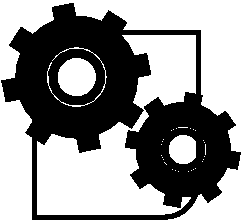
\includegraphics[width=0.75cm]{col11305.imgs/summary_simulation.png} &   \end{array} $ \hspace{2 pt}\raisebox{-5 pt}{} {(section shortcode: P10106 )} \par 
      \label{m38786*id68299}Mechanical energy, ${E}_{M}$, is simply the sum of gravitational potential energy (${E}_{P}$) and the kinetic energy (${E}_{K}$). Mechanical energy is defined as:\par 
      \label{m38786*uid76}\nopagebreak\noindent{}
    \begin{equation}
    {E}_{M}={E}_{P}+{E}_{K}
      \end{equation}
      \label{m38786*uid77}\nopagebreak\noindent{}
    \begin{equation}
    \begin{array}{ccc}\hfill {E}_{M}& =& {E}_{P}+{E}_{K}\hfill \\ \hfill {E}_{M}& =& mgh+\frac{1}{2}m{v}^{2}\hfill \end{array}
      \end{equation}
      \label{m38786*eip-384}
\Tip{You may see mechanical energy written as $U$. We will not use this notation in this book, but you should be aware that this notation is sometimes used.}
      \label{m38786*uid78}
            

\section{Conservation of mechanical energy}
            \nopagebreak
\Definition{ Conservation of Energy } { The Law of Conservation of Energy: Energy cannot be created or destroyed, but is merely changed from one form into another.  } 
        \label{m38786*id68483}So far we have looked at two types of energy: gravitational potential energy and kinetic energy. 
The sum of the gravitational potential energy and kinetic energy is called the mechanical energy. 
In a closed system, one where there are no external dissipative forces acting, the mechanical energy will remain constant. 
In other words, it will not change (become more or less). This is called the Law of Conservation of Mechanical Energy. 

\Definition{ Conservation of Mechanical Energy } { Law of Conservation of Mechanical Energy: The total amount of mechanical energy, in a closed system in the absence of dissipative forces (e.g. friction, air resistance), remains constant.  } 

This means that potential energy can become kinetic energy, or vice versa, but energy cannot 'disappear'. 
For example, in the absence of air resistance, the mechanical energy of an object moving through the air in the Earth's gravitational field, remains constant (is conserved).

\Tip{In problems involving the use of conservation of energy, the path taken by the object can be ignored. The only important quantities are the object's velocity (which gives its kinetic energy) and height above the reference point (which gives its gravitational potential energy).}


The following simulation covers the law of conservation of energy. \newline
    \setcounter{subfigure}{0}
	\begin{figure}[H] % horizontal\label{m38806*transverse-waves}
    \textnormal{Phet simulation for energy}\vspace{.1in} \nopagebreak
  \label{m38806*phet!!!underscore!!!sim}\label{m38806*phet-simulation}
            \raisebox{-5 pt}{ 
\includegraphics[width=0.5cm]{col11305.imgs/summary_www.png}} { (Simulation:  lTd )}
      \vspace{2pt}
    \vspace{.1in}
 \end{figure}       \par 
      \label{m38786*uid79}


\subsection*{Using the law of conservation of energy}
            \nopagebreak
        \label{m38786*id68660}Mechanical energy is conserved (in the absence of friction). Therefore we can say that the sum of the ${E}_{P}$ and the ${E}_{K}$ anywhere during the motion must be equal to the sum of the ${E}_{P}$ and the ${E}_{K}$ anywhere else in the motion.\par 
        \label{m38786*id68713}We can now apply this to the example of the suitcase on the cupboard. Consider the mechanical energy of the suitcase at the top and at the bottom. We can say:\par 
        \label{m38786*id68720}
    \setcounter{subfigure}{0}
\begin{figure}[H]
\begin{center}
\begin{pspicture}(0,0)(3,5)
%\psgrid[subgriddiv=1,griddots=10,gridlabels=7pt]
\psframe[linewidth=2pt](0,0)(2,4)
%suitcase on top
\psframe[linewidth=1.5pt](1.2,4)(2,4.5)
\pscurve[linewidth=2pt](1.4,4.5)(1.6,4.7)(1.8,4.5)
%suitcase at bottom
\psframe[linewidth=1.5pt](2.2,0)(3,0.5)
\pscurve[linewidth=2pt](2.4,0.5)(2.6,0.7)(2.8,0.5)
\psline[linestyle=dashed](2,4)(3,4)
\psline[linestyle=dotted]{->}(2.6,4)(2.6,0.8)
\rput[l](3.1,4){The mechanical energy ($E_{M}$) at the top.}
%\rput[l](3.1,-0.2){The kinetic energy is a maximum at the bottom}
\rput[l](3.2,2.8){The mechanical energy will remain}
\rput[l](3.2,2.4){constant throughout the motion.}
%\rput[l](3.1,4.2){The potential energy is a maximum at the top.}
\rput[l](3.1,0){The mechanical energy ($E_{M}$) at the bottom.}
\end{pspicture}
\end{center}
\end{figure}   
        \par 
        \label{m38786*id68729}\nopagebreak\noindent{}
    \begin{equation}
    \begin{array}{ccc}\hfill {E}_{\text{M 1}}& =& {E}_{\text{M 2}}\hfill \\ 
\hfill {E}_{\text{P 1}}+{E}_{\text{K 1}}& =& {E}_{\text{P 2}}+{E}_{\text{K 2}}\hfill \\ 
\hfill mgh+\frac{1}{2}m{v}^{2}& =& mgh+\frac{1}{2}m{v}^{2}\hfill \\ 
\hfill \left(1\right)\left(9,8\right)\left(2\right)+0& =& 0+\frac{1}{2}\left(1\right)\left({v}^{2}\right)\hfill \\ 
\hfill 19,6\phantom{\rule{3.33333pt}{0ex}}\text{J}& =& \frac{1}{2}{v}^{2}\hfill \\ 
\hfill 39,2& =& {v}^{2}\hfill \\ 
\hfill v& =& 6,26\phantom{\rule{0.166667em}{0ex}}\text{m}\ensuremath{\cdot}{\text{s}}^{-1}\hfill \end{array}
      \end{equation}
The suitcase will strike the ground with a velocity of $6,26\phantom{\rule{2pt}{0ex}}\text{m}\ensuremath{\cdot}\text{s}{}^{-1}$.\par 
From this we see that when an object is lifted, like the suitcase in our example, it gains potential energy. As it falls back to the ground, it will lose this potential energy, but gain kinetic energy. We know that energy cannot be created or destroyed, but only changed from one form into another. In our example, the potential energy that the suitcase loses is changed to kinetic energy.\par 
The suitcase will have maximum potential energy at the top of the cupboard and maximum kinetic energy at the bottom of the cupboard. Halfway down it will have half kinetic energy and half potential energy. As it moves down, the potential energy will be converted (changed) into kinetic energy until all the potential energy is gone and only kinetic energy is left. The $19,6\phantom{\rule{2pt}{0ex}}\text{J}$ of potential energy at the top will become $19,6\phantom{\rule{2pt}{0ex}}\text{J}$ of kinetic energy at the bottom.\par 

\begin{activity}{Conversion of energy}
\textbf{Materials:}\\
A length of plastic pipe with diameter approximately 20 mm, a marble, some masking tape and a measuring tape. \\
\textbf{To do (1):}\\
First put one end of the pipe on the table top so that it is parallel to the top of the table and tape it in position with the masking tape. \\
Lift the other end of the pipe upwards and hold it at a steady height not too high above the table. \\
Measure the vertical height from the table top to the top opening of the pipe. \\
Now put the marble at the top of the pipe and let it go so that it travels through the pipe and out the other end. \\ \\
\textbf{Questions:}\\ 
\begin{itemize}
\item What is the velocity (i.e. fast, slow, not moving) of the marble when you first put it into the top of the pipe and what does this mean for its gravitational potential and kinetic energy? 
\item What is the velocity (i.e. fast, slow, not moving) of the marble when it reaches the other end of the pipe and rolls onto the desk? What does this mean for its gravitational potential and kinetic energy?
\end{itemize}

\textbf{To do (2):}\\
Now lift the top of the pipe as high as it will go. \\
Measure the vertical height of the top of the pipe above the table top. \\
Put the marble into the top opening and let it roll through the pipe onto the table.\\
\textbf{Questions:}\\ 
\begin{itemize}
\item What is the velocity (i.e. fast, slow, not moving) of the marble when you put it into the top of the pipe, and what does this mean for its gravitational potential and kinetic energy?
\item Compared to the first attempt, what was different about the height of the top of the tube? How do you think this affects the gravitational potential energy of the marble?
\item Compared to your first attempt, was the marble moving faster or slower when it came out of the bottom of the pipe the second time? What does this mean for the kinetic energy of the marble?
\end{itemize}
\end{activity}

The activity with the marble rolling down the pipe shows very nicely the conversion between gravitational potential energy and kinetic energy. In the first instance, the pipe was held relatively low and therefore the gravitational potential energy was also relatively low. The kinetic energy at this point was zero since the marble wasn't moving yet. When the marble rolled out of the other end of the pipe, it was moving relatively slowly, and therefore its kinetic energy was also relatively low. At this point its gravitational potential energy was zero since it was at zero height above the table top. 

In the second instance, the marble started off higher up and therefore its gravitational potential energy was higher. By the time it got to the bottom of the pipe, its gravitational potential energy was zero (zero height above the table) but its kinetic energy was high since it was moving much faster than the first time. Therefore, the gravitational potential energy was converted completely to kinetic energy (if we ignore friction with the pipe). 

In the case of the pipe being held higher, the gravitational potential energy at the start was higher, and the kinetic energy (and velocity) of the marble was higher at the end. In other words, the total mechanical energy was higher and and only depended on the height you held the pipe above the table top and not on the distance the marble had to travel through the pipe. 


\label{m38786*secfhsst!!!underscore!!!id1898}\vspace{.5cm} 
      \noindent
\begin{wex}{Using the Law of Conservation of Mechanical Energy}{During a flood a tree trunk of mass 100 kg falls down a waterfall. The waterfall is 5 m high. If air resistance is ignored, calculate \begin{enumerate}[label=\textbf{\arabic*}.]
\item the potential energy of the tree trunk at the top of the waterfall.
\item the kinetic energy of the tree trunk at the bottom of the waterfall.
\item the magnitude of the velocity of the tree trunk at the bottom of the waterfall.
\end{enumerate}
\scalebox{1} % Change this value to rescale the drawing.
{
\begin{pspicture}(0,-1.787)(3.6098125,1.815)
\psline[linewidth=0.024cm](0.0978125,1.225)(1.7978125,1.225)
\psline[linewidth=0.024cm](1.7978125,1.225)(1.7978125,-1.775)
\psline[linewidth=0.024cm](1.7978125,-1.775)(3.5978124,-1.775)
\psline[linewidth=0.124cm](1.2978125,1.325)(1.8978125,1.325)
\psline[linewidth=0.124cm](1.8978125,-1.675)(2.4978125,-1.675)
\psline[linewidth=0.024cm,linestyle=dashed,dash=0.16cm 0.16cm,tbarsize=0.07055555cm 5.0,arrowsize=0.05291667cm 2.0,arrowlength=1.4,arrowinset=0.4]{|->}(2.7978125,1.225)(2.7978125,-1.775)
\rput(3.1684375,-0.065){5 m}
\rput(4.2,1.36){m = 100 kg}
%\usefont{T1}{ptm}{m}{n}
\rput(0.62,0.26){waterfall}
\end{pspicture} 
}
}
{\westep{Analyse the question to determine what information is provided}
\begin{itemize}
\item The mass of the tree trunk $m$ = 100~kg
\item The height of the waterfall $h$ = 5 m.
\\
These are all in SI units so we do not have to convert.
\end{itemize}

\westep{Analyse the question to determine what is being asked}
\begin{itemize}
\item Potential energy at the top
\item Kinetic energy at the bottom
\item Velocity at the bottom
\end{itemize}

\westep{Calculate the potential energy.}
\begin{eqnarray*}
E_{P} &=& mgh\\
&=& (100)(9,8)(5)\\
&=& 4900~\text{J}
\end{eqnarray*}

\westep{Calculate the kinetic energy.}
The kinetic energy of the tree trunk at the bottom of the waterfall is equal to the potential energy it had at the top of the waterfall. Therefore $E_{K}$ = 4900 J.\\

\westep{Calculate the velocity.}
To calculate the velocity of the tree trunk we need to use the equation for kinetic energy.
\begin{eqnarray*}
E_{K} & = & \frac{1}{2}mv^2 \\
4900 &=& \frac{1}{2} (100) (v^2) \\
98 &=& v^2\\
v &=& 9,899...\\
v &=& 9,90 \ \text{downwards}
\end{eqnarray*}}
\end{wex}
    \noindent
\par
            \label{m38786*secfhsst!!!underscore!!!id2130}\vspace{.5cm} 
      \noindent
\begin{wex}{Pendulum}{A 2~kg metal ball is suspended from a rope. If it is released from point $A$ and swings down to the point $B$ (the bottom of its arc): \begin{enumerate}[label=\textbf{\arabic*}.]
\item Show that the velocity of the ball is independent of it mass.
\item Calculate the velocity of the ball at point $B$.
\end{enumerate}
\begin{center}
\begin{pspicture}(-0.1,-0.3)(3.3,3.1)
%\psgrid
\psline{-}(3,3)(1.2,1)\psline{-}(3,3)(3,0.3)
\pscircle*(1.2,1){0.15}\pscircle*(3,0.3){0.15}
\psline[linestyle=dashed]{-}(0,0.3)(3.3,0.3)
\psline[linestyle=dashed]{-}(0,1)(1.5,1)
\psline{<->}(0.7,1)(0.7,0.3)
\rput(0.95,1.3){A}\rput(3,-0.05){B}
\rput(0.15,0.65){0.5m}
\end{pspicture}
\end{center}}
{\westep{Analyse the question to determine what information is provided}
\begin{itemize}
\item{The mass of the metal ball is $m$ = 2~kg}
\item{The change in height going from point $A$ to point $B$ is $h$ = 0,5~m}
\item{The ball is released from point $A$ so the velocity at point, $v_A$ = 0~\ms.}
\end{itemize}

All quantities are in SI units.\\

\westep{Analyse the question to determine what is being asked}
\begin{itemize}
\item Prove that the velocity is independent of mass.
\item Find the velocity of the metal ball at point $B$.
\end{itemize}

\westep{Apply the Law of Conservation of Mechanical Energy to the situation}
As there is no friction, mechanical energy is conserved. Therefore: 
\begin{eqnarray*}
E_{MA} &=& E_{MB}\\
E_{PA} + E_{KA} &=& E_{PB} + E_{KB}\\
mgh_A + \frac{1}{2}m(v_A)^2 &=& mgh_B + \frac{1}{2}m(v_B)^2\\
mgh_A + 0 &=& 0 + \frac{1}{2}m(v_B)^2\\
mgh_A &=& \frac{1}{2}m(v_B)^2
\end{eqnarray*}
As the mass of the ball $m$ appears on both sides of the equation, it can be eliminated so that the equation becomes:
$gh_A = \frac{1}{2}(v_B)^2}$
$2gh_A = (v_B)^2}$
This proves that the velocity of the ball is independent of its mass. It does not matter what its mass is, it will always have the same velocity when it falls through this height.
\westep{Calculate the velocity of the ball}
We can use the equation above, or do the calculation from 'first principles':
\begin{eqnarray*}
(v_B)^2 &=& 2gh_A\\
(v_B)^2 &=& (2)(9.8)(0,5)\\
(v_B)^2 &=& 9,8\\
v_B &=& \sqrt{9,8}~ \ \text{m} \cdot \text{s}^{-1}}
\end{eqnarray*}}
\end{wex}
    \noindent
\label{m38786*secfhsst!!!underscore!!!id2545}
\begin{exercises}{Potential Energy }
            \nopagebreak \noindent
            \label{m38786*id70623}\begin{enumerate}[noitemsep, label=\textbf{\arabic*}. ] 
            \label{m38786*uid95}\item A tennis ball, of mass $120\phantom{\rule{2pt}{0ex}}\text{g}$, is dropped from a height of $5\phantom{\rule{2pt}{0ex}}\text{m}$. Ignore air friction.
\label{m38786*id70639}\begin{enumerate}[noitemsep, label=\textbf{\alph*}. ] 
            \label{m38786*uid96}\item What is the potential energy of the ball when it has fallen $3\phantom{\rule{2pt}{0ex}}\text{m}$?
\label{m38786*uid97}\item What is the velocity of the ball when it hits the ground?
\end{enumerate}
                \label{m38786*uid98}\item A bullet, mass $50\phantom{\rule{2pt}{0ex}}\text{g}$, is shot vertically up in the air with a muzzle velocity of $200\phantom{\rule{2pt}{0ex}}\text{m}\ensuremath{\cdot}\text{s}{}^{-1}$. Use the Principle of Conservation of Mechanical Energy to determine the height that the bullet will reach. Ignore air friction.\newline
\label{m38786*uid99}\item A skier, mass $50\phantom{\rule{2pt}{0ex}}\text{kg}$, is at the top of a $6,4\phantom{\rule{2pt}{0ex}}\text{m}$ ski slope.
\label{m38786*id70721}\begin{enumerate}[noitemsep, label=\textbf{\alph*}. ] 
            \label{m38786*uid100}\item Determine the maximum velocity that she can reach when she skies to the bottom of the slope.
\label{m38786*uid101}\item Do you think that she will reach this velocity? Why/Why not?
\end{enumerate}
                \label{m38786*uid102}\item A pendulum bob of mass $1,5\phantom{\rule{2pt}{0ex}}\text{kg}$, swings from a height A to the bottom of its arc at B. The velocity of the bob at B is $4\phantom{\rule{2pt}{0ex}}\text{m}\ensuremath{\cdot}\text{s}{}^{-1}$. Calculate the height A from which the bob was released. Ignore the effects of air friction.\newline
\label{m38786*uid103}\item Prove that the velocity of an object, in free fall, in a closed system, is independent of its mass.\newline
\end{enumerate}
    \label{m38786*cid8}
\par \raisebox{-0.2em}{
\includegraphics[height=1em]{../icons/www.eps}} Find the answers with the shortcodes:
 \par \begin{tabular}[h]{cccccc}
 (1.) lxV  &  (2.) lxp  &  (3.) lxd  &  (4.) lxv  &  (5.) lxw  & \end{tabular}
\end{exercises}
            \section*{Summary}
            \nopagebreak
      \label{m38786*id70947}\begin{itemize}[noitemsep]
            \label{m38786*uid111}\item The potential energy of an object is the energy the object has due to his position above a reference point.
\label{m38786*uid112}\item The kinetic energy of an object is the energy the object has due to its motion.
\label{m38786*uid113}\item Mechanical energy of an object is the sum of the potential energy and kinetic energy of the object.
\label{m38786*uid114}\item The unit for energy is the joule (J).
\label{m38786*uid115}\item The Law of Conservation of Energy states that energy cannot be created or destroyed, but can only be changed from one form into another.
\label{m38786*uid116}\item The Law of Conservation of Mechanical Energy states that the total mechanical energy of an isolated system remains constant.
\label{m38786*uid117}\item The table below summarises the most important equations:
\end{itemize}
    % \textbf{m38786*id71092}\par
          \begin{table}[H]
    % \begin{table}[H]
    % \\ '' '0'
        \begin{center}
      \label{m38786*id71092}
    \noindent
      \begin{tabular}{|l|l|}\hline
        Potential Energy &
                ${E}_{P}=mgh$
             \\ \hline
        Kinetic Energy &
                ${E}_{K}=\frac{1}{2}m{v}^{2}$
              \\ \hline
        Mechanical Energy &
                ${E}_{M}={E}_{K}+{E}_{P}$
            \\ \hline
    \end{tabular}
      \end{center}
\end{table}
    \par
\begin{table}[H]
\begin{center}
\begin{tabular}{|l|c|c|c|}\hline \hline 
\multicolumn{4}{|c|}{\textbf{Units}}\\ \hline \hline
\textbf{Quantity} & \textbf{Symbol} & \textbf{Unit} & \textbf{S.I. Units}\\ \hline
Potential energy & $E_{P}$ & J & $\text{kg} \cdot \text{m}^{2} \cdot \text{s}^{-2}$ \\ \hline
Kinetic energy & $E_{K}$ & J & $\text{kg} \cdot \text{m}^{2} \cdot \text{s}^{-2}$ \\ \hline
Mechanical energy & $E_{M}$ & J & $\text{kg} \cdot \text{m}^{2} \cdot \text{s}^{-2}$ \\ \hline
\end{tabular}
\end{center}
\caption{Units used in \textbf{mechanical energy} }
\label{table:electricity::units}
\end{table}
    \label{m38786*cid9}
\begin{eocexercises}{Mechanical Energy}
            \nopagebreak
      \label{m38786*id71520}\begin{enumerate}[noitemsep, label=\textbf{\arabic*}. ] 
            \label{m38786*uid118}\item Give one word/term for the following descriptions.
\label{m38786*id71536}\begin{enumerate}[noitemsep, label=\textbf{\alph*}. ] 
            \label{m38786*uid119}\item The force with which the Earth attracts a body.
\label{m38786*uid120}\item The unit for energy.
\label{m38786*uid121}\item The movement of a body in the Earth's gravitational field when no other forces act on it.
\label{m38786*uid122}\item The sum of the potential and kinetic energy of a body.
\label{m38786*uid123}\item The amount of matter an object is made up of.
\end{enumerate}
                \label{m38786*uid124}\item Consider the situation where an apple falls from a tree. Indicate whether the following statements regarding this situation are TRUE or FALSE. Write only 'true' or 'false'. If the statement is false, write down the correct statement.
\label{m38786*id71616}\begin{enumerate}[noitemsep, label=\textbf{\alph*}. ] 
            \label{m38786*uid125}\item The potential energy of the apple is a maximum when the apple lands on the ground.
\label{m38786*uid126}\item The kinetic energy remains constant throughout the motion.
\label{m38786*uid127}\item To calculate the potential energy of the apple we need the mass of the apple and the height of the tree.
\label{m38786*uid128}\item The mechanical energy is a maximum only at the beginning of the motion.
\label{m38786*uid129}\item The apple falls at an acceleration of $9,8\phantom{\rule{2pt}{0ex}}\text{m}\ensuremath{\cdot}\text{s}{}^{-2}$.
\end{enumerate}
                \label{m38786*uid131}\item A man fires a rock out of a slingshot directly upward. The rock has an initial velocity of $15\phantom{\rule{2pt}{0ex}}\text{m}\ensuremath{\cdot}\text{s}{}^{-1}$.
\label{m38786*id71971}\begin{enumerate}[noitemsep, label=\textbf{\alph*}. ] 
            \label{m38786*uid133}\item What is the maximum height that the rock will reach?
\label{m38786*uid134}\item Draw graphs to show how the potential energy, kinetic energy and mechanical energy of the rock changes as it moves to its highest point.
\end{enumerate}
                  \label{m38786*uid135}\item A metal ball of mass $200\phantom{\rule{2pt}{0ex}}\text{g}$ is tied to a light string to make a pendulum. The ball is pulled to the side to a height (A), $10\phantom{\rule{2pt}{0ex}}\text{cm}$ above the lowest point of the swing (B). Air friction and the mass of the string can be ignored. The ball is let go to swing freely.
\label{m38786*id72026}\begin{enumerate}[noitemsep, label=\textbf{\alph*}. ] 
            \label{m38786*uid136}\item Calculate the potential energy of the ball at point A.
\label{m38786*uid137}\item Calculate the kinetic energy of the ball at point B.
\label{m38786*uid138}\item What is the maximum velocity that the ball will reach during its motion?
\end{enumerate}
                \label{m38786*uid139}\item A truck of mass $1,2\phantom{\rule{2pt}{0ex}}\text{tons}$ is parked at the top of a hill, $150\phantom{\rule{2pt}{0ex}}\text{m}$ high. The truck driver lets the truck run freely down the hill to the bottom.
\label{m38786*id72082}\begin{enumerate}[noitemsep, label=\textbf{\alph*}. ] 
            \label{m38786*uid140}\item What is the maximum velocity that the truck can achieve at the bottom of the hill?
\label{m38786*uid141}\item Will the truck achieve this velocity? Why/why not?
\end{enumerate}
                \label{m38786*uid142}\item A stone is dropped from a window, $6\phantom{\rule{2pt}{0ex}}\text{m}$ above the ground. The mass of the stone is $25\phantom{\rule{2pt}{0ex}}\text{g}$.
Use the Principle of Conservation of Energy to determine the speed with which the stone strikes the ground.
           \end{enumerate}
  \label{m38786**end}
  \label{1fc5ba69690764517c30802fdf7b1905**end}
\par \raisebox{-0.2em}{
\includegraphics[height=1em]{../icons/www.eps}} Find the answers with the shortcodes:
 \par \begin{tabular}[h]{cccccc}
 (1.) lxf  &  (2.) lxG  &  (3.) lbW  &  (4.) lxo  &  (5.) lxs  &  (6.) lbZ  & \end{tabular}
\end{eocexercises}
